\subsection{Observations and Motivation} % just find the problem and benefit
\label{sec:observationandmotivation}



\paragraph{Deduplication for improving storage capacity.}

On-cloud global deduplication software is widely adopted by cloud enterprises for reducing cloud storage consumption and overall storage cost. 
For example, StorReduce~\cite{storReduce}, the deduplication software used by
Google cloud and AWS, 
performs in-line transparent data deduplication. StorReduce resides between the client's application and the hosting cloud storage.
%A number of deduplication methods focus on client-side data deduplication to ensure that only unique files are uploaded, 
%to save network bandwidth, by having the client send a duplicate check request~\cite{xxx}~\cite{xxx}. 
%For example, xxxx\NZ{Hadeel, can you add one example and few relatedwork citation?}. 
Intuitively, such deduplication techniques can be leveraged to eliminate redundant data from the Docker image storage system.  
Except, the Docker image dataset is not amenable to deduplication 
as the images are \emph{compressed archival files}.
%Intuitively, registries can be deployed as a proxy cache to host frequently requested layers to speedup image pulls and improve performance 
%while the backend cloud storage can leverage deduplication to save storage space.
%However, there are several unique problems concerning the integration of caching and deduplication to the unique Docker registries workload: \textbf{compressed layers}. 
%We investigate the potential for data reduction in the Docker registry by estimating the efficacy of layer sharing and file-level deduplication.
%We noticed that the number of public repositories is constantly increasing with a growth that amounts 
%to around 1 million repositories annually. 
%This corresponds to~130\,TB of annual growth in storage needs 
%\HA{but it is actually less because of shared layers, right?}, 
%costing around~\$15,000 a month if Google Cloud Storage is used~\cite{GoogleCloudStoragePricing}.
%This growth implies significant benefits to data deduplication. 


As discussed in~\cref{sec:intro}, only $\~3\%$ of the files in a sample Docker hub image collection were found to be unique, mainly becuase 
 compressed files have a very low deduplication ratio~\cite{meister2012study}.
Thus, 
we can save realize significant space savings if we can remove the 
duplicate files. This entails decompressing files before performing deduplication, and collecting components of layers from multiple servers.
%
To quantify the performance overhead of such an approach involving decompressing, deduplication, and then re-compressing,
we setup five registry instances. Each instance has a local file system as their backend storage system. We
implemented file-level deduplication with decompression and compression operations.
We replayed the IBM registry workload \texttt{dal}~\cite{dockerworkload} 
%by sending requests randomly 
randomly to our five registries and measured the latency. 
%
Figure~\ref{fig:avg_latency_dedup_nodedup} shows the average latency observed \arb{average across what??}.
Note that since 
%the IBM registry workload 
\texttt{dal} does not contain real layers,
we extract the layer digest from each request and match it with a layer randomly selected from our Docker Hub dataset to emulate realistic registry requests.

Without deduplication,
the average latency for requesting a layer is about 2~s for layers with sizes less than~50~MB.
The latency increases to 12~s when the above deduplication is implemented in the backend storage system.
Furthermore, Docker registry performance drops down dramatically for larger layers.
We observe that the average latency for requesting layers larger than 50~MB and smaller than 1~GB
is about 128~s. The latency worsens when dedupliation is implemented, to on average about 800~s.

%\HA{running five registries, replaying dal trace using trace replayer-cite, and since the replayer doesn't use real layers we randomly match the request to our dataset downloaded from docker hub. describe how we got these numbers. for dedup, we simply implemented a decompress/compress + file-level deduplication on backend storage systems, we use a CHT based distributed storage system. Figure~\ref{fig:avg_latency_dedup_nodedup}}
\begin{figure}[t]
	\centering
	%\scriptsize
	\begin{minipage}{0.225\textwidth}
		\centering
		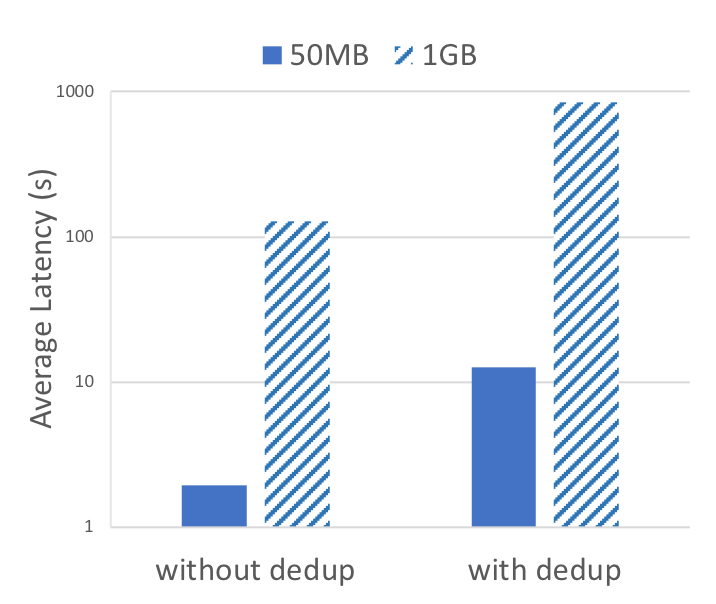
\includegraphics[width=1\textwidth]{graphs/avglatency_dedup_nodedup.png}
		\caption{Average latency.}
		\label{fig:avg_latency_dedup_nodedup}
	\end{minipage}
	\begin{minipage}{0.225\textwidth}
		\centering
		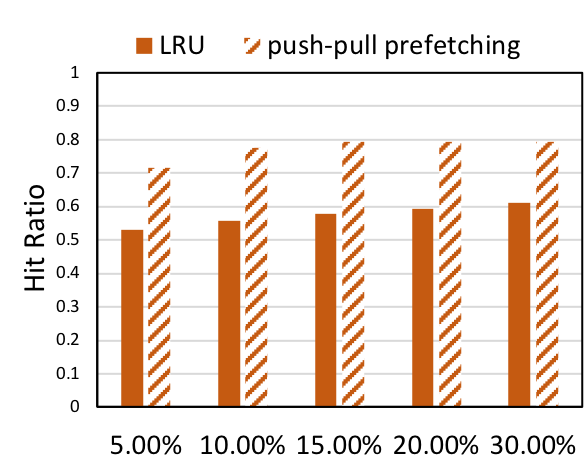
\includegraphics[width=1\textwidth]{graphs/lru_prefetch_hits.png}
		\caption{Hit ratio.}
		\vspace{-3pt}
		\label{fig:lru_prefetching_hits}
	\end{minipage}
\end{figure}
% for LRU and push-pull prefetching under different cache sizes (\% of total accessed layers).

\paragraph{Registry as a cache for improving performance.}
Traditionally, caches are placed as close to the requesting client as possible. 
Such caches are known as proxy caches, or web/HTTP caches for the temporary storage of 
frequently requested data to mitigate the remote server lag. 
For example, Varnish~\cite{varnish} and Squid~\cite{squid} are high-performance web/HTTP caches that accelerate web applications and improve response times by caching frequently requested web content.
%Examples of open-source web (HTTP) proxy caches include Nginx~\cite{?}, Squid~\cite{?}, and Varnish~\cite{?}. 
%They are typically implemented in an regional ISP or within a corporate network.
%Deduplication methods are implemented on remote backend storage servers, and
%transparently remove duplicates from the incoming data stream and restore the data for read requests. 
Docker registry is a web server that serves docker \texttt{pull} and docker \texttt{push} requests.
Intuitively, registries can be deployed as proxy caches, \ie a pull-through cache~\cite{registryascache}, to host frequently requested layers. This will speedup image pulls and improve performance. 

However, the layer access pattern differs greatly from traditional request streams.
Traditional LRU will place recently requested data into the cache 
because it is highly likely that the data will be requested again.
However, it is the opposite for the layer access pattern: if a layer is pulled by a user,
then this layer will not be pulled by the same user in the future
since the layer is now locally available to the user. Thus, we have to design innovative mechanisms to manage any caches.

\begin{figure}[t]
	\centering
		\begin{minipage}{0.225\textwidth}
			\centering
			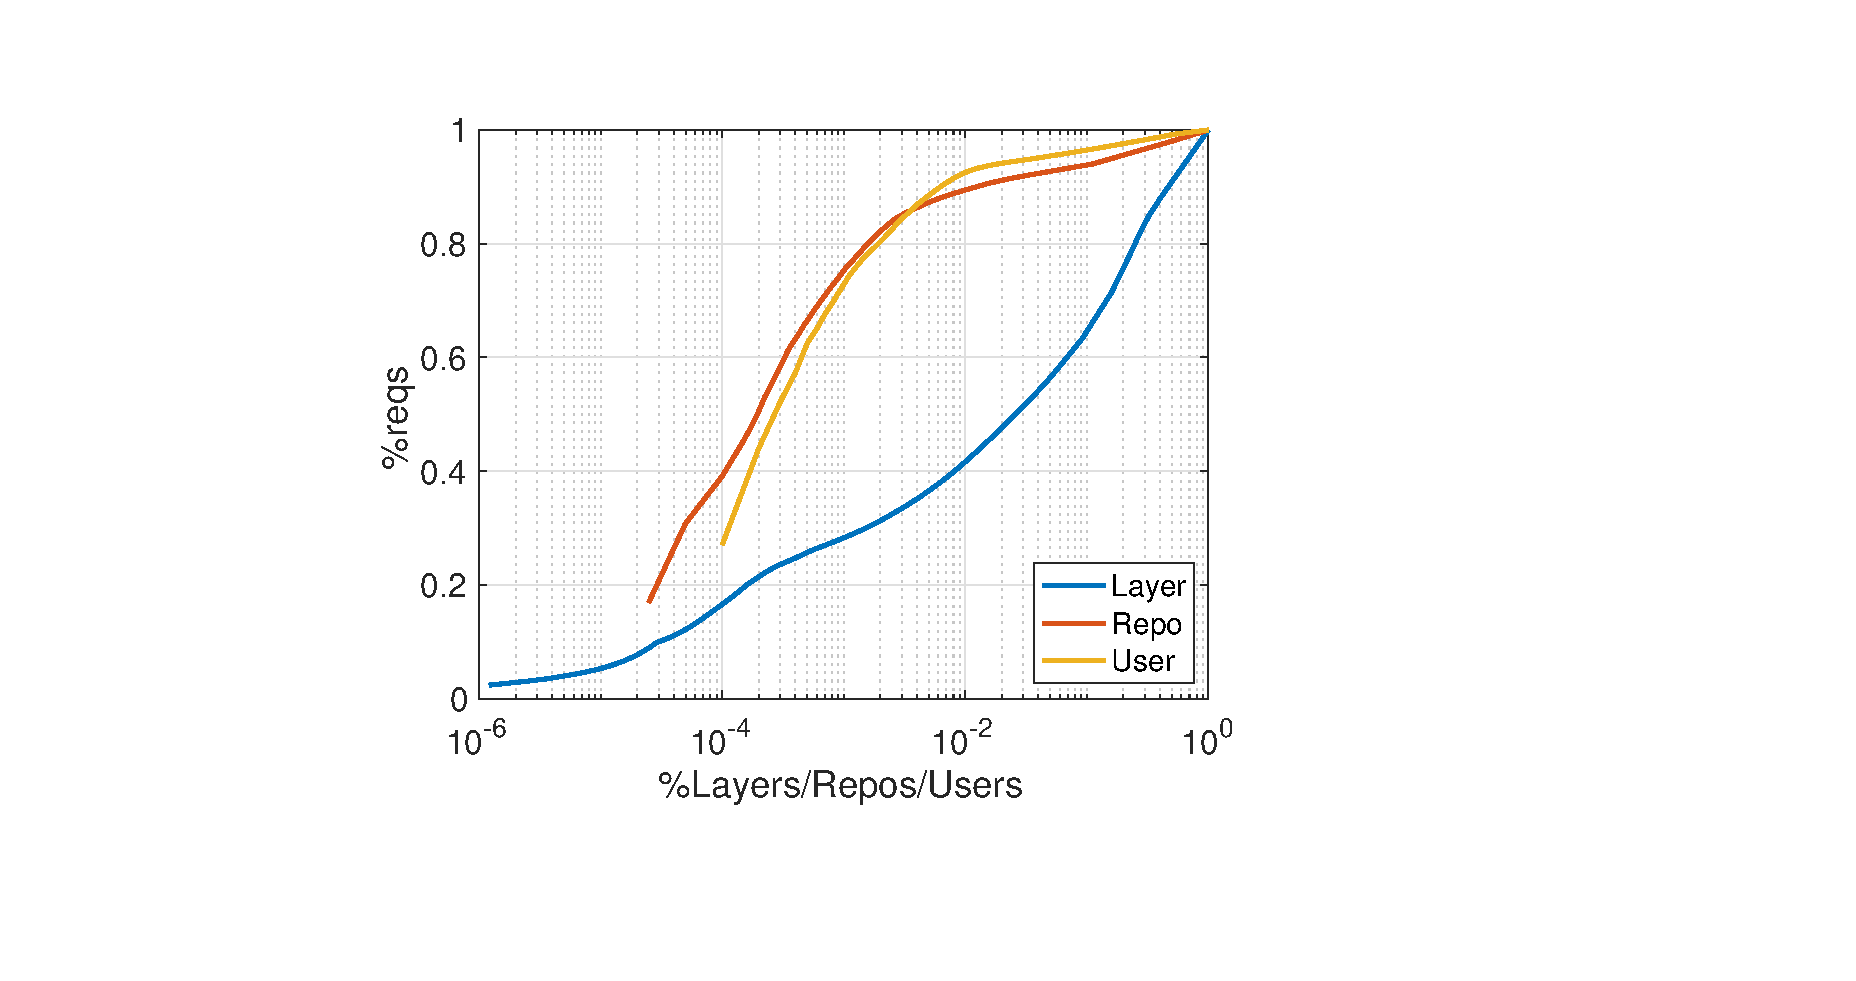
\includegraphics[width=1\textwidth]{graphs/skewness_cdf.eps}
			\caption{Popularity of layers, repos, and users.}
			\label{fig:sknewss}
		\end{minipage}
	\begin{minipage}{0.225\textwidth}
		\centering
		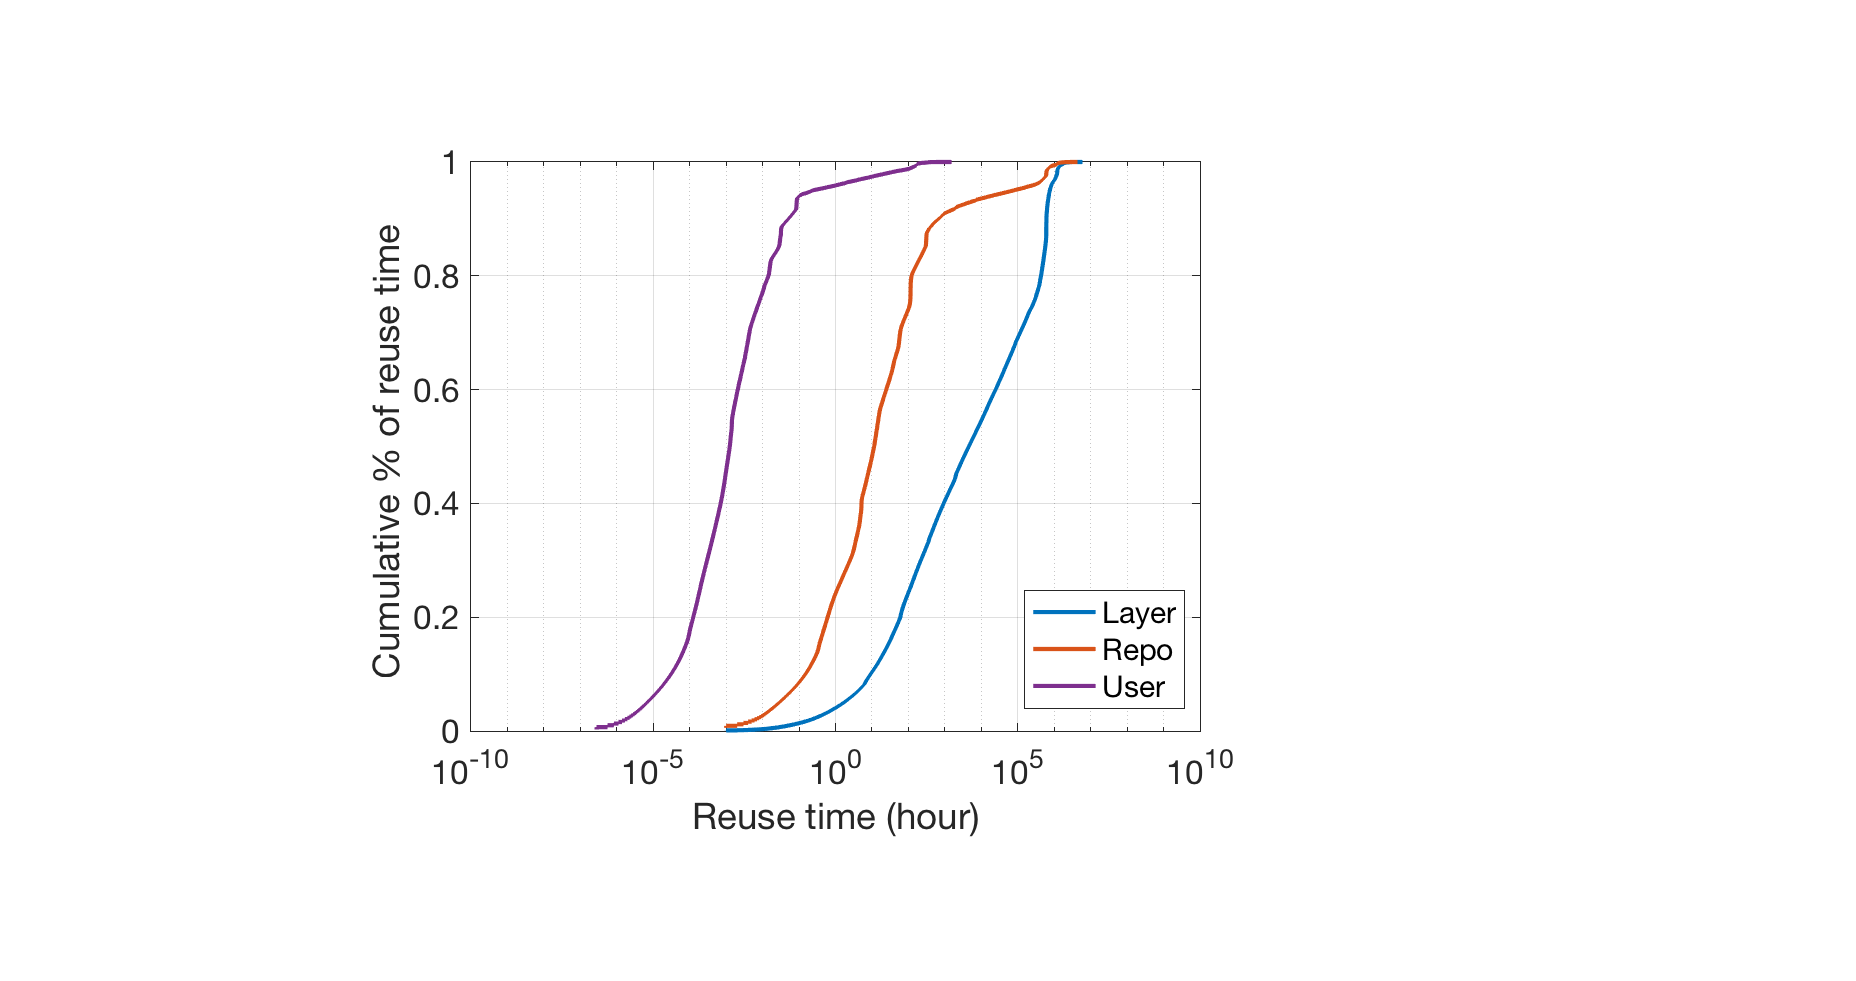
\includegraphics[width=1\textwidth]{graphs/reuse_time.eps}
		\caption{CDF of reuse time for layers, repos, and users.}
		\vspace{-3pt}
		\label{fig:reusetime}
	\end{minipage}
\end{figure}


%We analyzed IBM registry workload and made the two following obervations:
%Caching is a technique widely leveraged to reduce bandwidth and load off of highly loaded bottleneck backends by temporarily storing frequently requested data~\cite{xxx}. 
%Caching can be introduced at the client, in between clients and servers as a proxy, or at the server side. 
%Proxy caches are efficient in reducing traffic from bottleneck backends by cooperatively serving previously requested and saved data without it going all they way to the backend~\cite{xxxx}. 
%Usually, caches are placed as close to the requesting client as possible, 
%such caches are known as proxy caches, or web/HTTP caches for the short-lived storage of 
%frequently requested/accessed data to reduce the server's lag. 

%The client therefore, experiences improved response times.
%The Docker client inherently caches layers at the client. This way, the Docker daemon only pulls layers that are not available on the host machine. 

%Other software used for caching include Memcached~\cite{?}, an open-source distributed in-memory key-value store that works as a caching system and Redis~\cite{?} which is an open-source key-value store that works as an in-memory store and as a cache
%\subsection{Apply traditional deduplication approaches to registries?}
%\subsection{Use-cases of \sysname}
%This suggests that the current layer sharing strategy that Docker already employs is not efficient in eliminating duplicate data. 
%Further investigations on the causes for the high number of redundant files exposed a few findings. 
%For example, different Docker images often contain the same 
%source code from external public repositories like GitHub~\cite{github}.
%This is because no official images contain this source code, 
%so users manually add it to their images, 
%resulting in different layers which cannot be reused.
%\paragraph{Deduplication statistics} % the potential of deduplication 

%%%%layer ref count 
%
%A remarkable observation that emerges from the data analysis is that only around 3\%\HA{3\% or 7\% ?} of the layers' constituent files are unique while the rest are redundant copies. 
%This suggests that the current layer sharing strategy that Docker already employs is not efficient in eliminating duplicate data. 
%We further analyzed the repeat count for every file and plotted the distributions as shown in Figure~\ref{fig:file-repeat-cnt}.
%We found that over 99.4\% of files have more than one copy.
%Around 50\% of files have exactly 4 copies and 90\% of files have 10 or less copies. 
%This indicates the high potential for file-level deduplication in the Docker registry.
%
%%\begin{figure} \centering
%	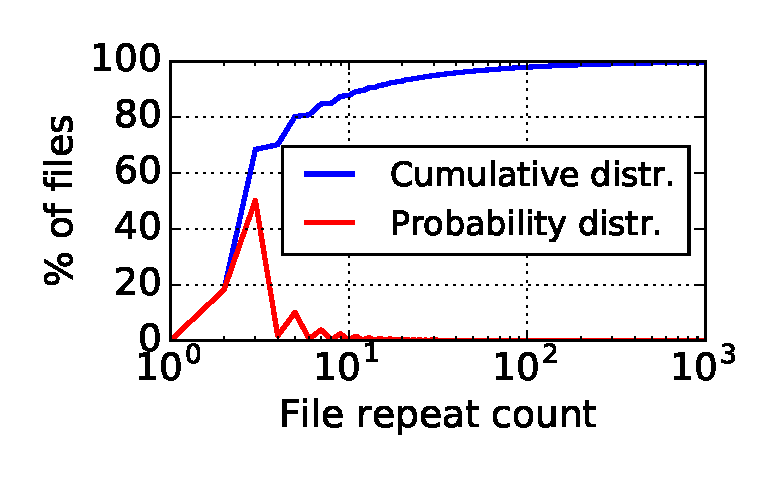
\includegraphics[width=0.45\textwidth]{graphs/File_repeat_count.eps}
%	\caption{File repeat count distribution.
%	%
%	\VT{No need for Y2}
%	%
%	\VT{Still need to use \% on the axis}\NZ{addressed both}
%	%
%	} \label{fig:file-repeat-cnt}
%\end{figure}

\begin{figure}[t]
	\centering
	\begin{minipage}{0.35\textwidth}
		\centering
		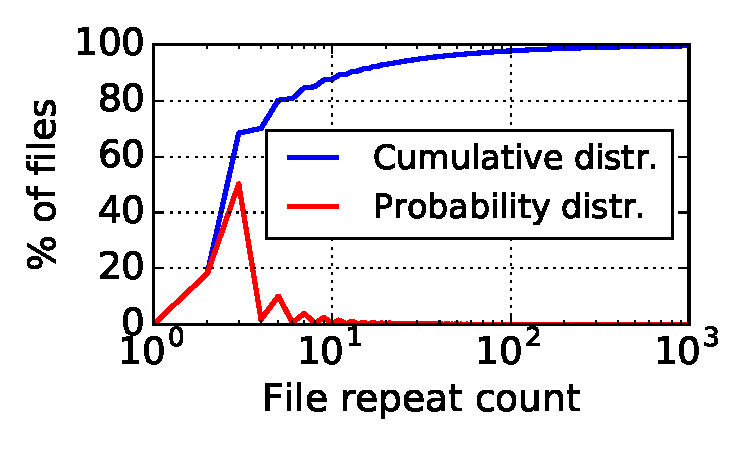
\includegraphics[width=1\textwidth]{graphs/File_repeat_count-eps.pdf}
		\caption{File repeat count distribution.
		}
		%\vspace{15pt}
		\label{fig:file-repeat-cnt}
	\end{minipage}
	\begin{minipage}{0.35\textwidth}
		\centering
		%\vspace{-10pt}
		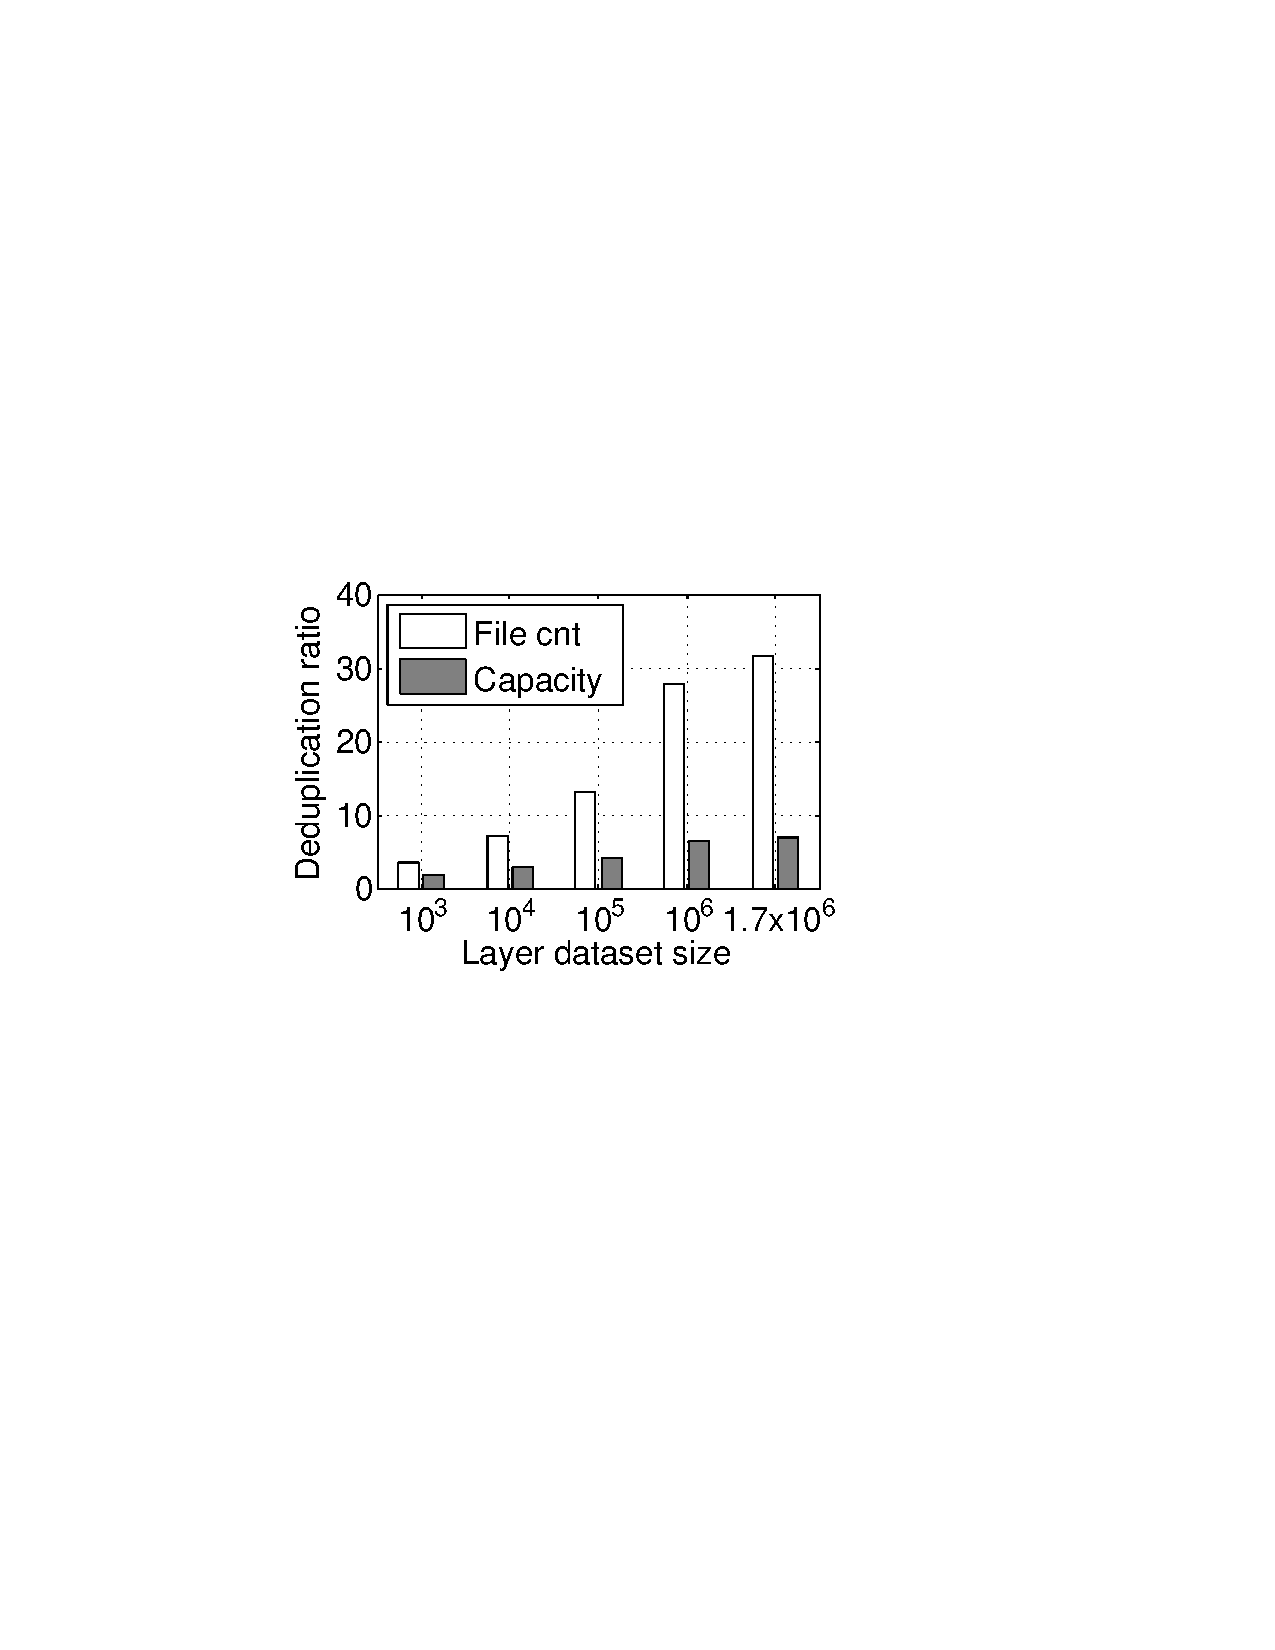
\includegraphics[width=1\textwidth]{graphs/dedup-ratio-grow} 
		\caption{Deduplication ratio growth.
		} 
		\vspace{-2pt}
		\label{fig:dedup-ratio-growth}
	\end{minipage}
\end{figure}

%\begin{figure} 
%	\centering
%	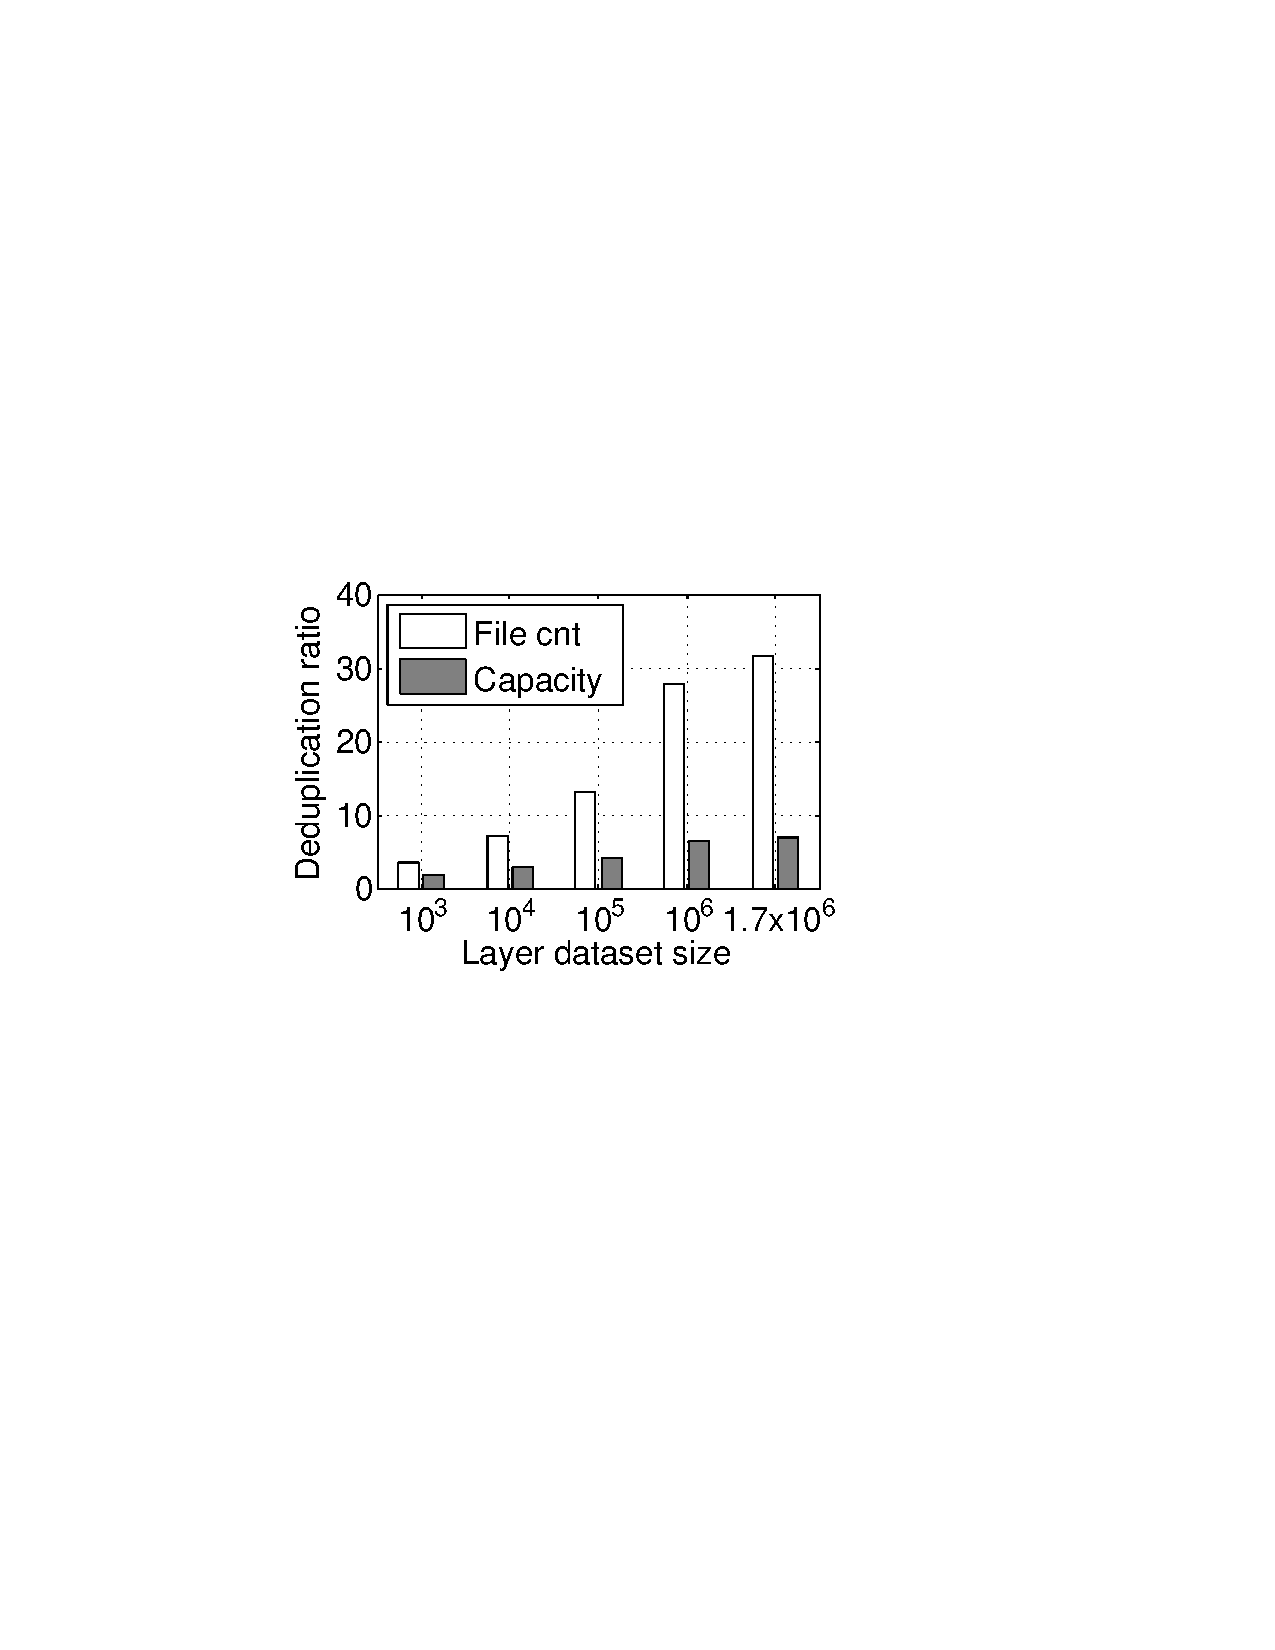
\includegraphics[width=0.25\textwidth]{graphs/dedup-ratio-grow} 
%	\caption{The growth of deduplication ratio.
%	} 
%	\label{fig:dedup-ratio-growth} 
%\end{figure}

%
%
%\paragraph{Deduplication ratio growth} % benefit
%%
%Further investigations on the potential of file-level deduplication involved analyzing the deduplication ratio. 
%As shown in Figure~\ref{fig:dedup-ratio-growth}, we analyzed the deduplication 
%ratio and its growth for an increasing number of files stored in the registry.   
%%(see Figure~\ref{fig:dedup-ratio-growth}).
%%
%%Figure~\ref{fig:dedup-ratio-growth} shows the deduplication ratio growth over the layer dataset size. 
%%
%The x-axis values correspond to the sizes of 4 random samples drawn from the whole dataset and the size of the
%whole dataset.
%
%We see that the deduplication ratio increases almost linearly with the layer dataset size.
%This implies that the benefits of file-level deduplication strengthens as the number of public repositories and images grow.
%
%As the number of images stored in the Docker registry increases dramatically,
%file-level deduplication can provide significant storage space savings.

%Intuitively, registries can be deployed as a proxy cache to host frequently requested layers to speedup image pulls and improve performance 
%while the backend cloud storage can leverage deduplication to save storage space.
%However, there are several unique problems concerning the integration of caching and deduplication to the unique Docker registries workload: \textbf{compressed layers}. 

%\subsection{Need for Usr-oriented cache management}
%
%\paragraph{Access skewness}
%
%\paragraph{Reuse time distribution}
%
%\paragraph{Hit ratios}
%
%\paragraph{Hit ratios with prefetching}
%
%%\subsection{} % what are the cost for a naive file-level deduplication
%
%\paragraph{Restoring performance breakdown}
